\documentclass[aspectratio=169,10pt,t]{beamer}
% \usetheme[
% %%% options passed to the outer theme
% %    progressstyle=fixedCircCnt,   %either fixedCircCnt, movCircCnt, or corner
% %    rotationcw,          % change the rotation direction from counter-clockwise to clockwise
% %    shownavsym          % show the navigation symbols
%   ]{SDUsimple}
\usepackage{SDUtheme/beamerthemeSDUsimple}
% If you want to change the colors of the various elements in the theme, edit and uncomment the following lines
% Change the bar and sidebar colors:
%\setbeamercolor{SDUsimple}{fg=red!20,bg=red}
%\setbeamercolor{sidebar}{bg=red!20}
% Change the color of the structural elements:
%\setbeamercolor{structure}{fg=red}
% Change the frame title text color:
%\setbeamercolor{frametitle}{fg=blue}
% Change the normal text color background:
%\setbeamercolor{normal text}{fg=black,bg=gray!10}
% ... and you can of course change a lot more - see the beamer user manual.
\usepackage{color}
\usepackage{float}
\usepackage{dsfont}                         % Enables double stroke fonts
\usepackage{bm}
\usepackage[utf8]{inputenc}
\usepackage[english]{babel}
\usepackage[T1]{fontenc}
\usepackage{listings}
% Or whatever. Note that the encoding and the font should match. If T1
% does not look nice, try deleting the line with the fontenc.
\usepackage{helvet}
\usefonttheme{professionalfonts}

\newtheorem{algorithm}{Algorithm}
%\newtheorem{problem}{Problem}
\newtheorem{proposition}{Proposition}
% colored hyperlinks
\newcommand{\chref}[2]{%
  \href{#1}{{\usebeamercolor[bg]{SDUsimple}#2}}%
}

\title{Covariance Structure and Dimension Reduction PCA}
\subtitle{Multivariate Statistic}
%\date{\today}
\date{ }

\author{
	Made by: \\
	\textbf{Lasse Gøransson, Marc Evald, Anne-Charlotte Poulsen \& Aske Møller}
}

% - Give the names in the same order as they appear in the paper.
% - Use the \inst{?} command only if the authors have different
%   affiliation. See the beamer manual for an example

\institute[
%  {\includegraphics[scale=0.2]{SDU_segl}}\\ %insert a company, department or university logo
  SDU Robotics\\
  The Maersk Mc-Kinney Moller Institute\\
  University of Southern Denmark
] % optional - is placed in the bottom of the sidebar on every slide
{% is placed on the bottom of the title page
  SDU Robotics\\
  The Maersk Mc-Kinney Moller Institute\\
  University of Southern Denmark

  %there must be an empty line above this line - otherwise some unwanted space is added between the university and the country (I do not know why;( )
}

% specify a logo on the titlepage (you can specify additional logos an include them in
% institute command below
\pgfdeclareimage[height=0.5cm]{titlepagelogo}{SDUgraphics/SDU_logo_new} % placed on the title page
%\pgfdeclareimage[height=1.5cm]{titlepagelogo2}{SDUgraphics/SDU_logo_new} % placed on the title page
\titlegraphic{% is placed on the bottom of the title page
  \pgfuseimage{titlepagelogo}
%  \hspace{1cm}\pgfuseimage{titlepagelogo2}
}

\begin{document}
% the titlepage
{\SDUwavesbg%
\begin{frame}[plain,noframenumbering] % the plain option removes the header from the title page
  \titlepage
\end{frame}}
%%%%%%%%%%%%%%%%

\begin{frame}[t]
    \frametitle{Agenda}
    \begin{itemize}
        \item Motivation
        \item Principal Components
        \item Variance
        \item Sample Based
        \item Pitfalls
    \end{itemize}

\end{frame}

\begin{frame}[t]
	\frametitle{Motivation}

    \begin{itemize}
        \item Dimension reduction
        \item Decorrelate data
    \end{itemize}

\end{frame}

\begin{frame}[t]
    \frametitle{Principal Components}
    
    \begin{align*}
        PC_i &\overset{def}{=} e_i_1 X_1 + \hdots + e_i_p X_p = e_i^T X\\
    \end{align*}

    \pause

    \begin{itemize}
        \item Maximize variance
    \end{itemize}
\end{frame}

\begin{frame}[t]
    \frametitle{Variance Explained}
    
    \begin{align*}
    \Sigma =  E\Lambda E^T
    \end{align*}

    \begin{align*}
    PC_i: \frac{\lambda_i}{ \sum^{p}_{j=1} \lambda_j  }
    \end{align*}
    
    
\end{frame}

\begin{frame}[t]
    \frametitle{Visualization}

    \begin{figure}[H]
        \centering
        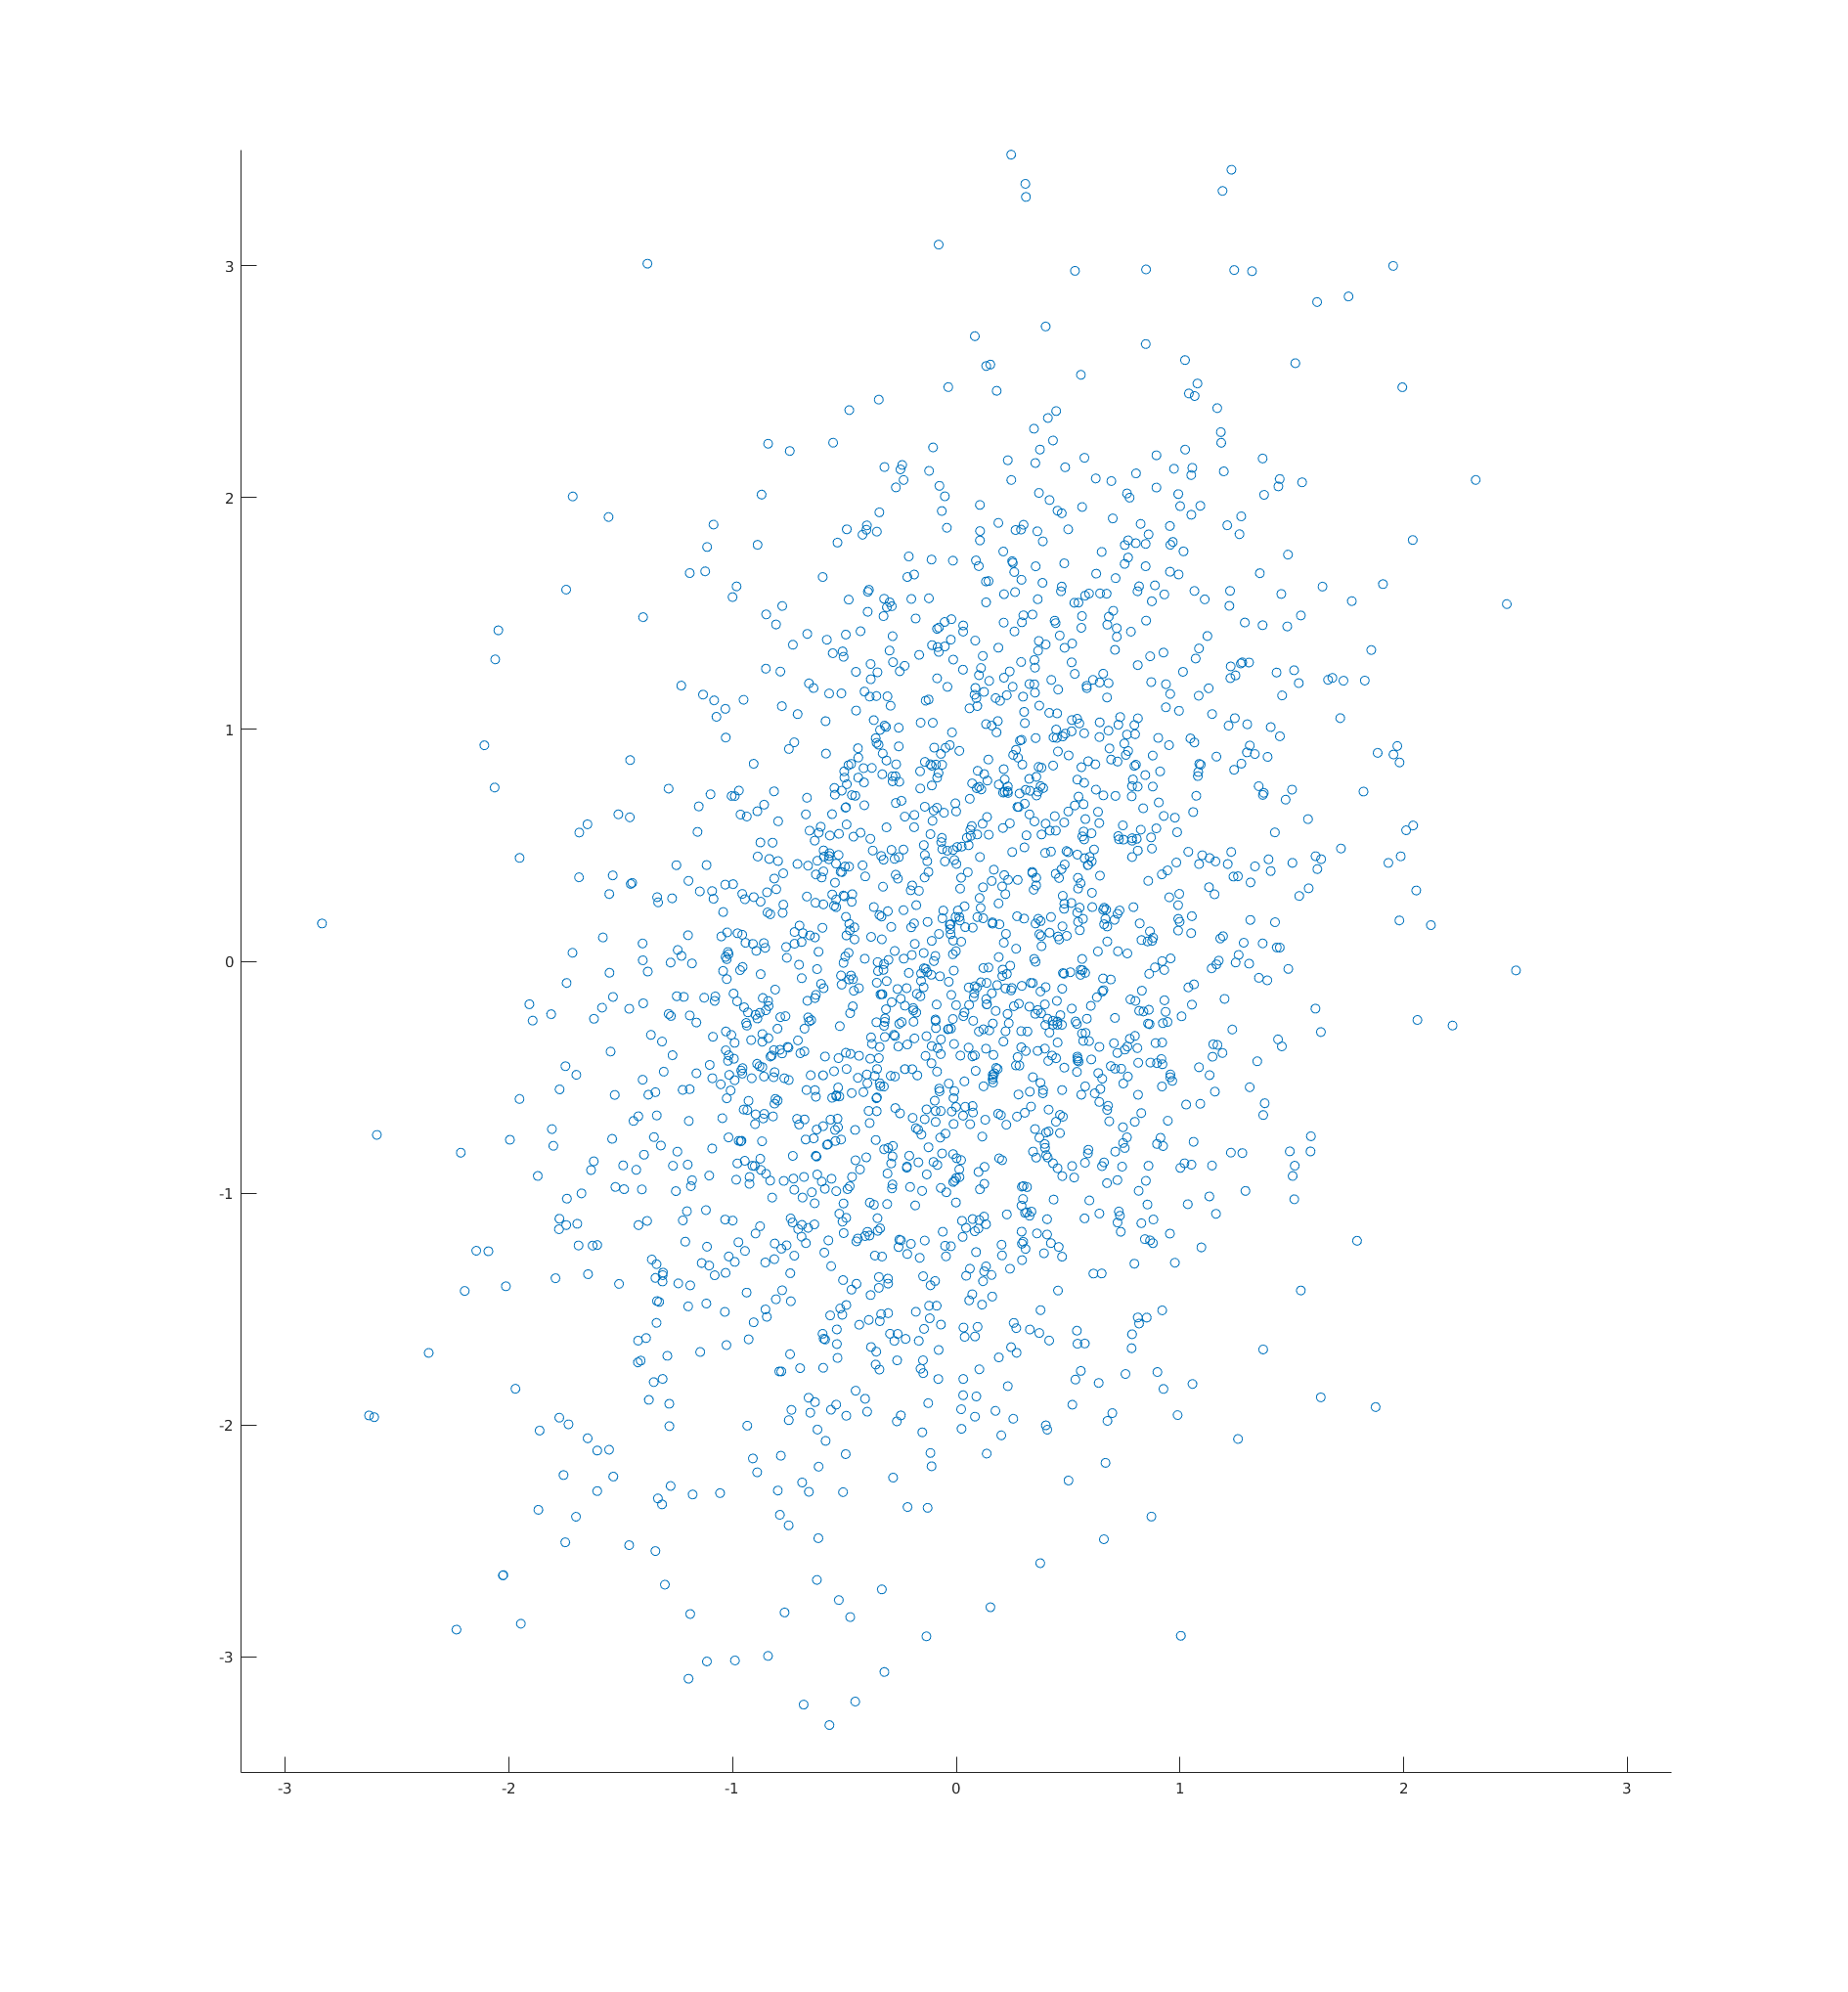
\includegraphics[width=0.45\linewidth]{images/pca.png}
    \end{figure}


    
\end{frame}
\begin{frame}[t]
    \frametitle{Visualization}

    \begin{figure}[H]
        \centering
        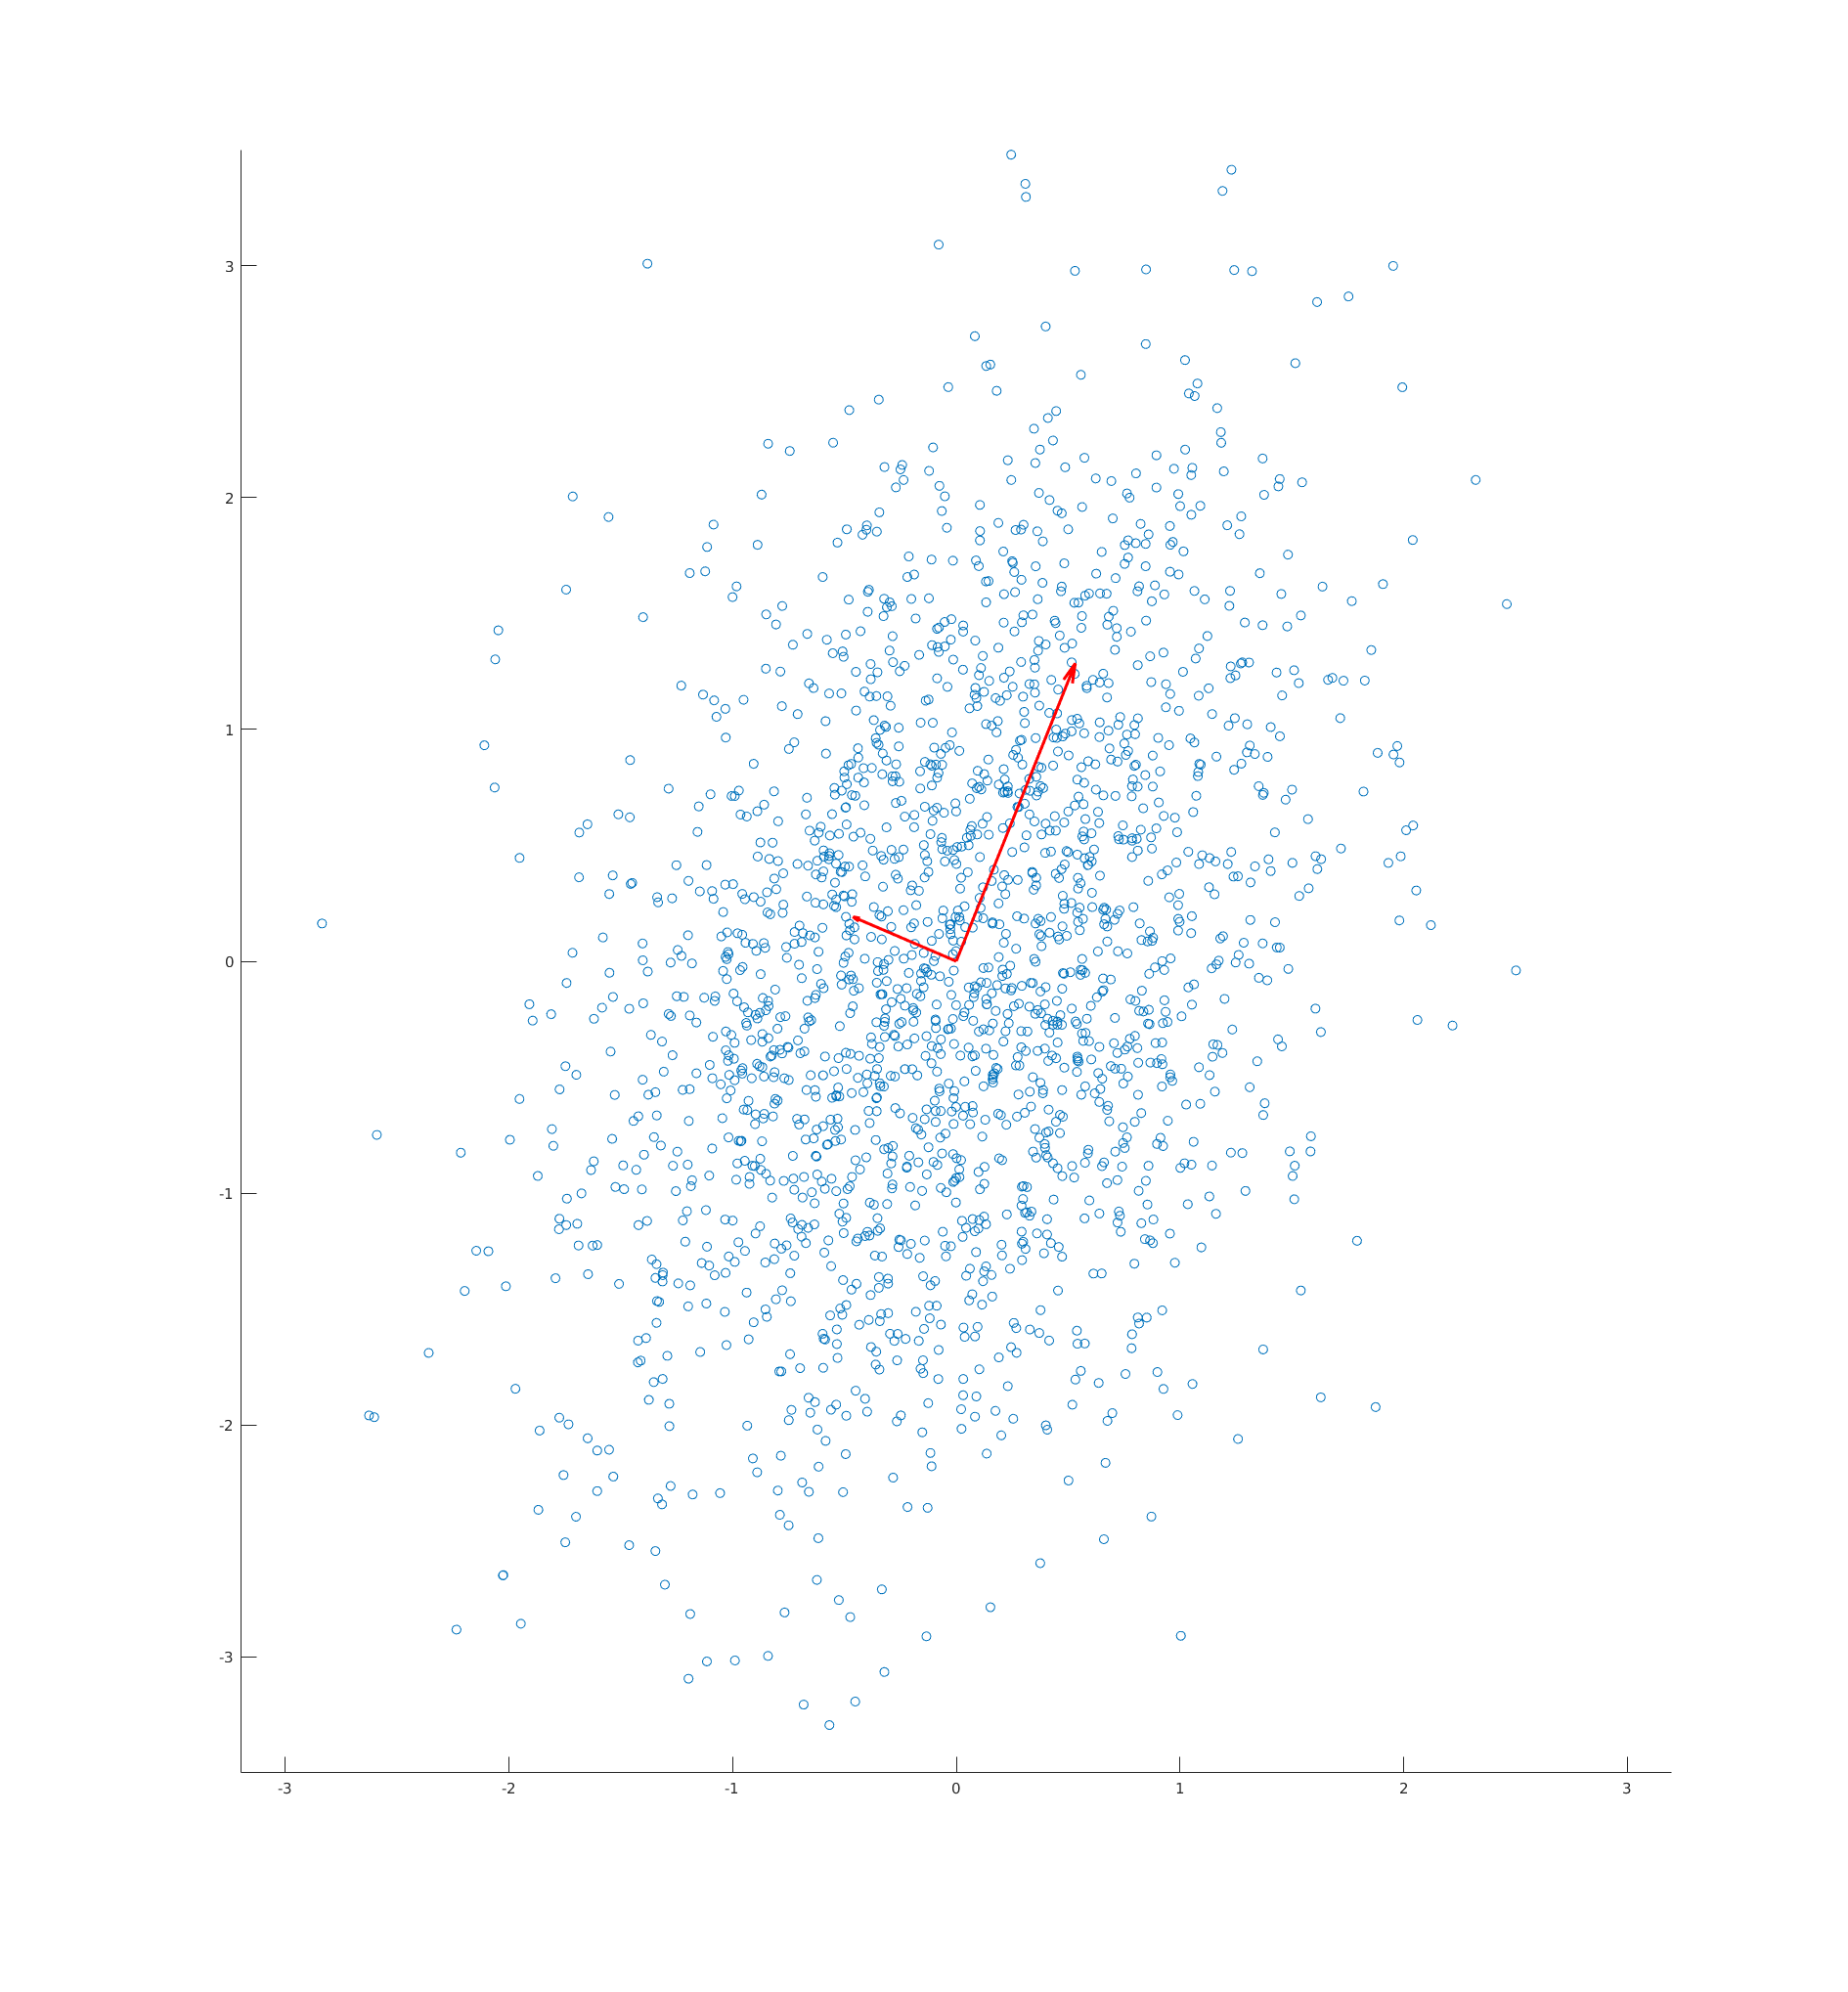
\includegraphics[width=0.45\linewidth]{images/pcaArrow.png}
    \end{figure}
    
\end{frame}

\begin{frame}[t]
    \frametitle{Sample Based}

    \begin{align*}
    X = \begin{bmatrix}
        X_1_1 & \hdots & X_1_p \\
        \vdots &  \ddots & \vdots  \\
        X_j_1 & \hdots & X_j_p \\
    \end{bmatrix}
    \end{align*}

    \begin{align*}
        \hat{\Sigma} = S = \frac{1}{n-1} \sum^{n}_{j=1} (X_j - \bar{X} )(X_j - \bar{X} )^T
    \end{align*}
   \begin{align*}
    \frac{ \sum^{r}_{i=1} \hat{\lambda_i}  }{ \sum^{p}_{j=1} \hat{\lambda_j}  }
   \end{align*}
    

    
\end{frame}

\begin{frame}[t]
    \frametitle{Pitfalls}

    \begin{align*}
    X = \begin{bmatrix}
        X_1_1 & \hdots & X_1_p \\
        \vdots &  \ddots & \vdots  \\
        X_j_1 & \hdots & X_j_p \\
    \end{bmatrix}
    \end{align*}

    
\end{frame}

\begin{frame}[t]
    \frametitle{Pitfalls}

    \begin{figure}[H]
        \centering
        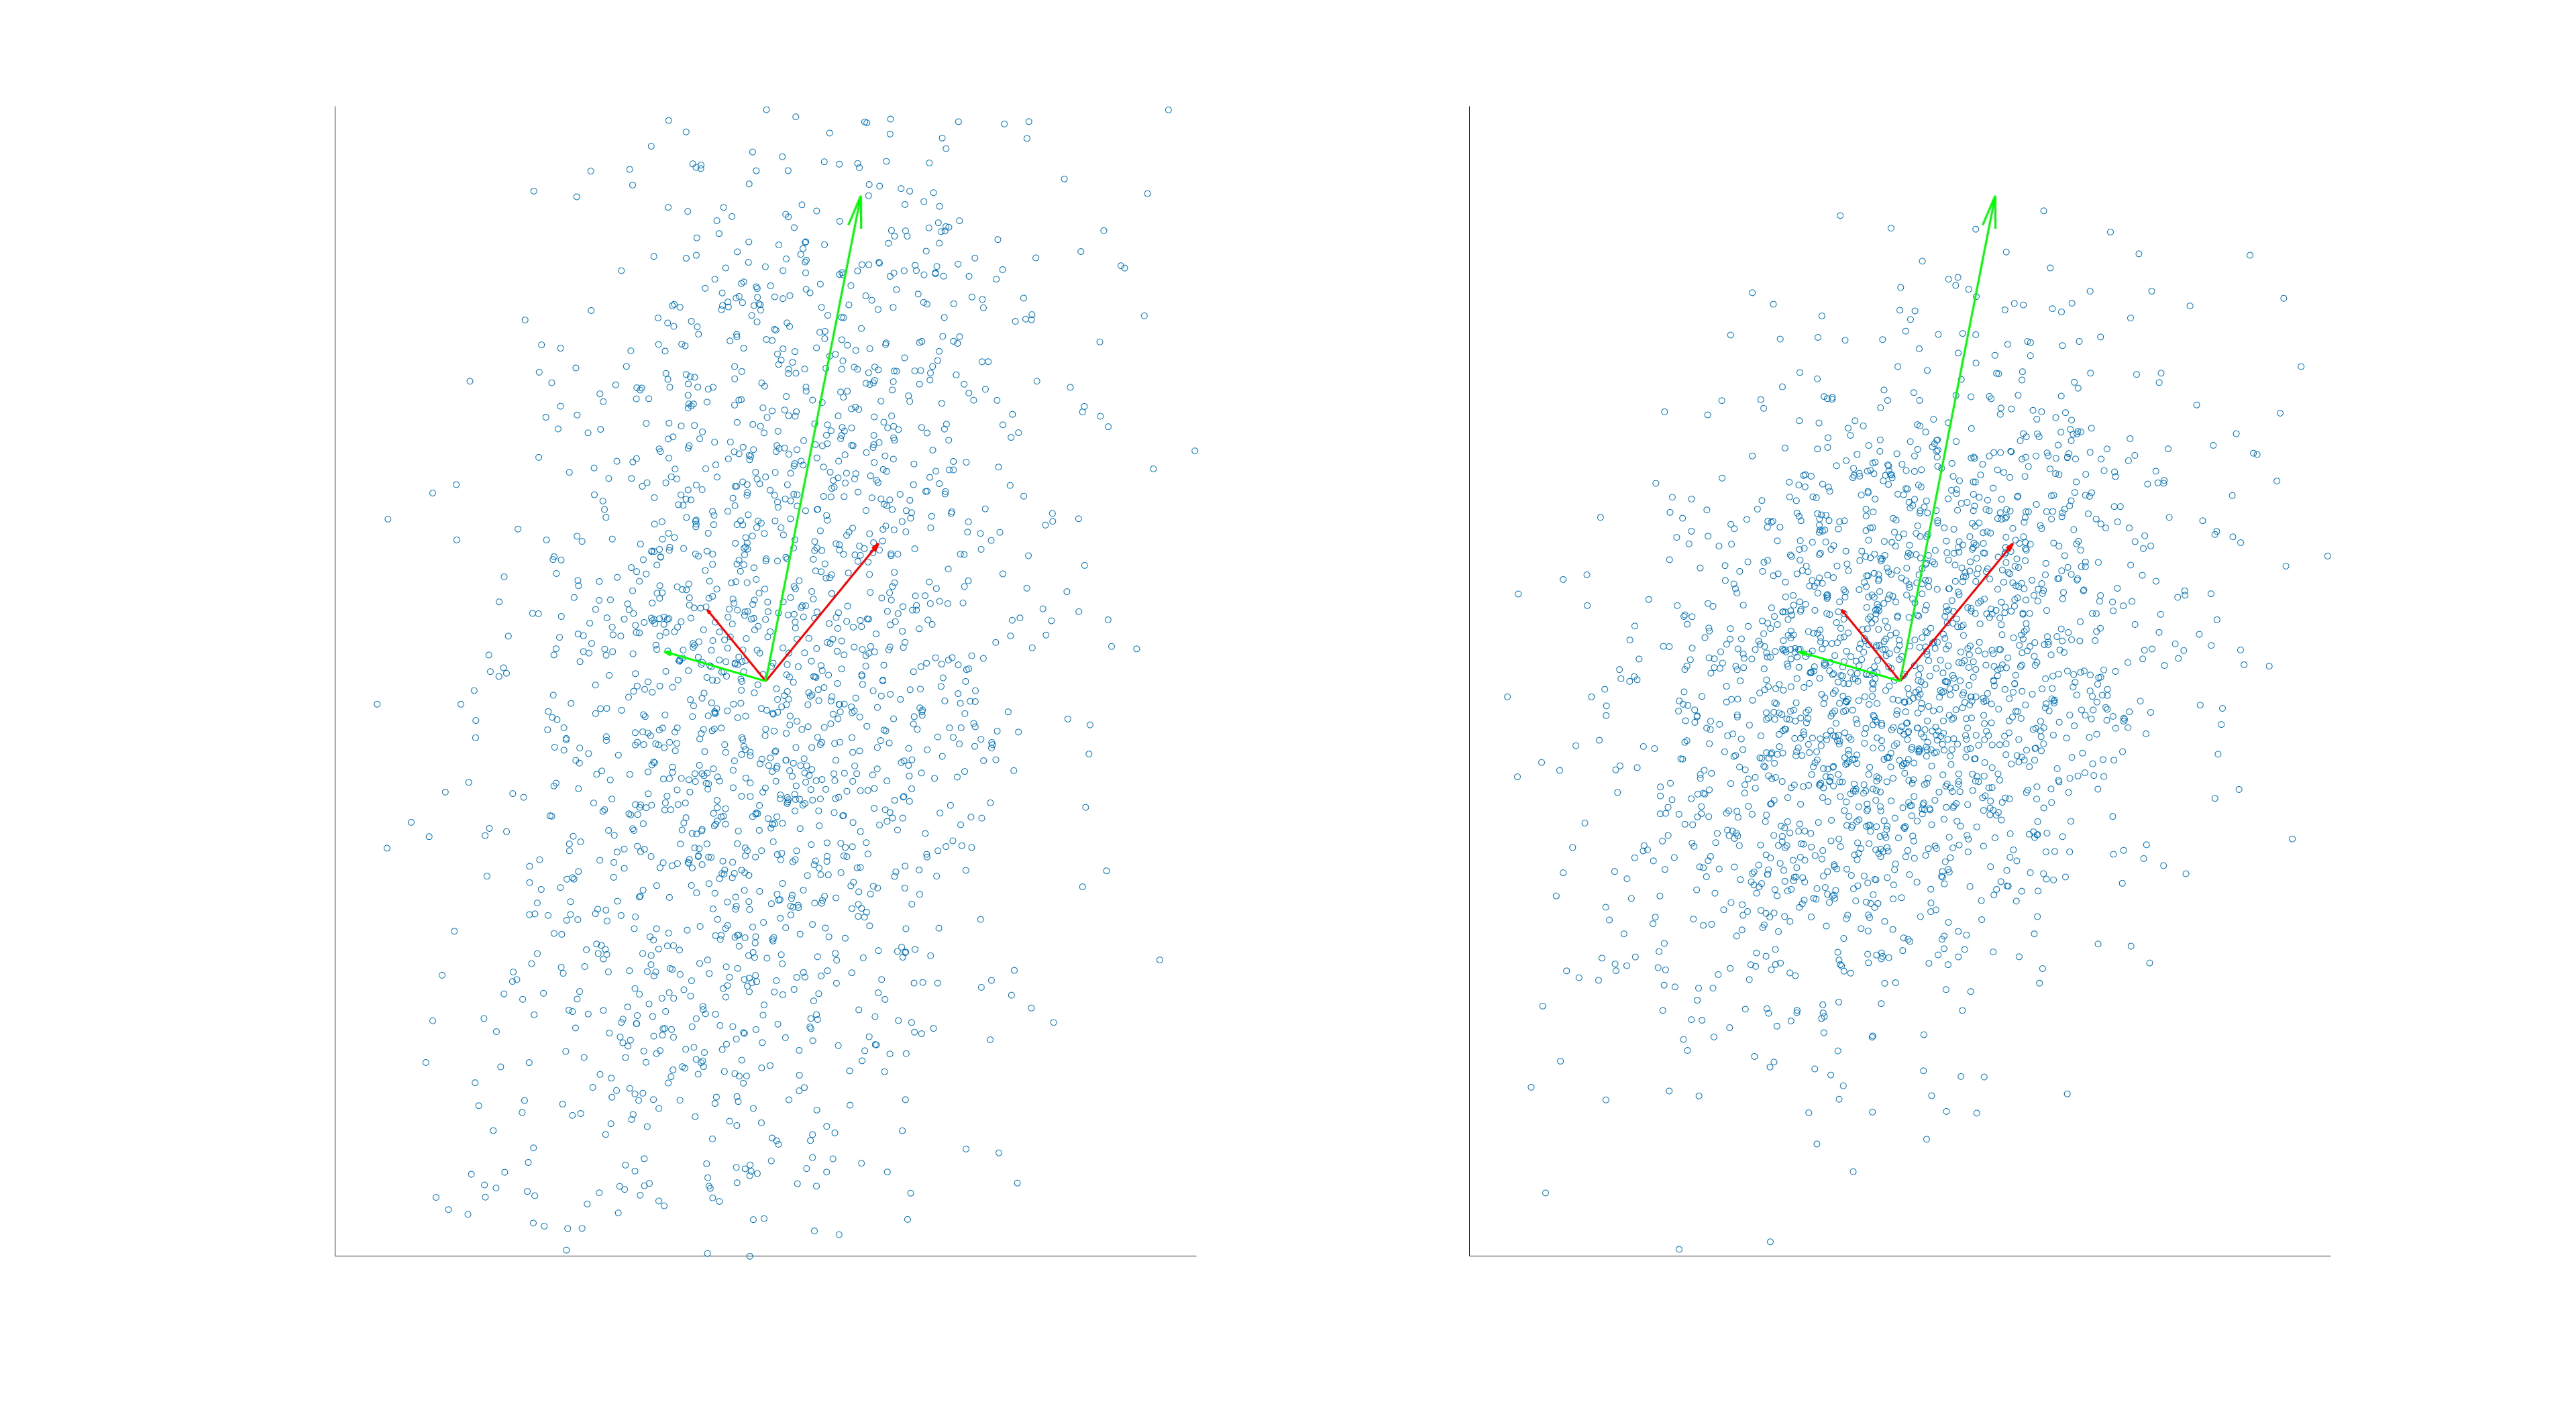
\includegraphics[width=0.8\linewidth]{images/compare.png}
    \end{figure}
    
\end{frame}

\begin{frame}[t]
    \frametitle{Inference}
    
    \begin{align*}
        \hat{\lambda_i} \sim N\left(\lambda_i,2\frac{\lambda_i^2}{n}\right) 
    \end{align*}
    \begin{align*}
        \frac{ \hat{\lambda_i}  }{1+ \sqrt{ \frac{2}{n} } z_{\frac{\alpha }{2}}} < \lambda_i < \frac{ \hat{\lambda_i}  }{1- \sqrt{ \frac{2}{n} } z_{\frac{\alpha }{2}}}
    \end{align*}
    
    

\end{frame}

\end{document}
